%==================================================================================================
\chapter{Formulação numérica para dinâmica não linear dos sólidos} \label{EGDS}
%==================================================================================================

Inicialmente considere um corpo deformável, idealizado como um meio contínuo que, em sua configuração inicial é denotado por $\Omega_0$ e em sua configuração atual é denotado por $\Omega$, conforme ilustrado na Figura \ref{fig:Cont}. Para se mapear os pontos que compõem o corpo em relação a uma origem preestabelecida utiliza-se $\BB{x}$ e $\BB{y}$ para denotar as coordenadas de $\Omega_0$ e $\Omega$, respectivamente. Já para se mapear $\BB{y}$ em função de $\BB{x}$ existe uma função $\BB{f}$ tal que $\BB{y}=\BB{f}(\BB{x})$, denominada como função de mudança de configuração.

\begin{figure}[h!]
    \centering
    \caption{Configurações inicial e atual de um corpo deformável.}
    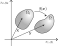
\includegraphics[width=.4\linewidth]{Figuras/Cont.pdf}
    \\Fonte: Autoria Própria (\the\year).
    \label{fig:Cont}
\end{figure}

Para um ponto $\BB{x}$ na vizinhança de $\BB{x}_0$, pode-se dizer que:

\begin{equation}
    \BB{y}(\BB{x})=\BB{f}(\BB{x}_0)+\left.\der{\BB{f}}{\BB{x}}\right|_{\BB{x}_0}\cdot d\BB{x}\text{,}
\end{equation}

\noindent em que $\BB{A}=\partial\BB{f}/\partial\BB{x}=\Nx\BB{f}$ é o gradiente de mudança de configuração. Assim, pode-se obter uma expressão que transforme um vetor $d\BB{x}$ na configuração inicial em um vetor $d\BB{y}$ na atual:

\begin{equation}
    d\BB{y}=\BB{A}\cdot d\BB{x}\text{,}\label{eq:dyAdx}
\end{equation}

\noindent o que permite escrever o quadrado da norma de $d\BB{y}$ como:

\[
    \norm{d\BB{y}}^2=dy^2=d\BB{y}^T\cdot d\BB{y}=(\BB{A}\cdot d\BB{x})^T\cdot(\BB{A}\cdot d\BB{x})=d\BB{x}^T\cdot\BB{A}^T\cdot\BB{A}\cdot d\BB{x}
\]

Subtraindo-se $dx^2=\norm{d\BB{x}}^2$ de ambos os lados da igualdade obtém-se:

\begin{equation}
    dy^2-dx^2=d\BB{x}^T\cdot(\BB{A}^T\cdot\BB{A}-\BB{I})\cdot d\BB{x}\text{,}
    \label{eq:difdxdy}
\end{equation}

\noindent em que $\BB{I}$ é o tensor identidade de segunda ordem e $\BB{C}=\BB{A}^T\cdot\BB{A}$ é o tensor de alongamento à direita de Cauchy-Green. Dessa maneira, pode-se substituir $\BB{C}$ em \eqref{eq:difdxdy} e dividir por $2dx^2$, obtendo-se:

\[
    \frac{1}{2}\frac{dy^2-dx^2}{dx^2}=\frac{1}{2}\frac{d\BB{x}^T\cdot(\BB{C}-\BB{I})\cdot d\BB{x}}{dx^2}\text{.}
\]

\noindent Tomando um versor na direção de $d\BB{x}$ ($\BB{u}=d\BB{x}/\norm{d\BB{x}}$), tem-se que:

\begin{equation}
    \frac{1}{2}\frac{dy^2-dx^2}{dx^2}=\BB{u}^T\cdot\left(\frac{1}{2}(\BB{C}-\BB{I})\right)\cdot\BB{u}\text{.}
\end{equation}

Assim, define-se o tensor de deformações de Green-Lagrange como:

\begin{equation}
    \mathbb{E}=\frac{1}{2}(\BB{C}-\BB{I})\text{,}
    \label{eq:CSD-DefGreenLagr}
\end{equation}

\noindent que se trata de uma medida de deformação objetiva, ou seja, não registra deformações em situação de movimento de corpo rígido.

Outra medida de deformação interessante é a medida de deformação volumétrica ($\varepsilon_V$). Para isso considere o elemento infinitesimal em suas configurações inicial e atual ilustrado na Figura \ref{fig:MudVol}.

\begin{figure}[h!]
    \centering
    \caption{Mudança de volume de um elemento infinitesimal.}
    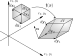
\includegraphics[width=0.5\linewidth]{Figuras/MudVol.pdf}
    \\Fonte: Autoria Própria (\the\year).
    \label{fig:MudVol}
\end{figure}

Logo o valor de $\varepsilon_V$ pode ser obtido através da relação entre o volume inicial e atual desse elemento como:

\begin{equation}
    \varepsilon_V=\frac{dV-dV_0}{dV_0}\text{.}
\end{equation}

O volume do elemento em ambas as configurações pode ser obtido por meio do produto misto dos vetores que formam o mesmo, ou seja:

\begin{subequations}
    \begin{equation}
        dV_0=d\BB{x}_1\cdot(d \BB{x}_2\times d\BB{x}_3)\text{,}
    \end{equation}
    \begin{equation}
        dV=d\BB{y}_1\cdot(d \BB{y}_2\times d\BB{y}_3)\text{,}
    \end{equation}
\end{subequations}

Conhecendo a transformação expressa em \eqref{eq:dyAdx} e fazendo as devidas simplificações pode-se obter que:

\begin{equation}
    dV=\det{(\BB{A})}dV_0=JdV_0\text{,}\label{eq:RelVol}
\end{equation}

\noindent em que $J=\det{(\BB{A})}$ é o Jacobiano da mudança de configuração.

Na sequência procura-se obter uma expressão que indique a mudança de área nas diferentes configurações. Assim, considere um cilindro infinitesimal ilustrado na figura \ref{fig:Nanson}.

\begin{figure}[h!]
    \centering
    \caption{Mudança de configuração em um cilindro infinitesimal.}
    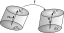
\includegraphics[width=.45\linewidth]{Figuras/Nanson.pdf}
    \\Fonte: Autoria Própria (\the\year).
    \label{fig:Nanson}
\end{figure}

Nesse contexto, a área vetorial pode ser entendida como seu valor absoluto na direção de sua normal ($d\BB{A}_0=dA_0\BB{N}$ e $d\BB{A}=dA\BB{n}$). Logo o volume do cilindro é dado pelo produto escalar da área vetorial com o vetor que define a altura do cilindro ($dV_0=d\BB{A}_0\cdot\BB{u}$ e $dV=\BB{A}\cdot\BB{v}$). Conhecendo as relações \eqref{eq:dyAdx} e \eqref{eq:RelVol}, pode-se obter que:

\begin{equation}
    \BB{n}dA=J\BB{A}^{-T}\cdot\BB{N}dA_0\text{,}\label{eq:Nanson}
\end{equation}

\noindent que é conhecida como a Equação de Nanson.

Com esse embasamento é possível apresentar os conceitos de energia nas descrições Euleriana e Lagrangiana Total. Assim, para se obter a equação do equilíbrio local de um elemento na descrição Euleriana, considere um elemento infinitesimal sujeito à ação de uma força de corpo (ou de volume) $\BB{c}$, conforme ilustrado no diagrama de corpo livre da Figura \ref{fig:CorpoLivreSolido}, que apresenta somente as forças atuantes na direção $y_1$.

\begin{figure}[h!]
    \centering
    \caption{Forças atuantes em um elemento infinitesimal na direção $y_1$.}
    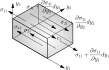
\includegraphics[width=.5\linewidth]{Figuras/CorpoLivreSolido.pdf}
    \\Fonte: Autoria Própria (\the\year).
    \label{fig:CorpoLivreSolido}
\end{figure}

Fazendo o equilíbrio das forças nessa direção e realizando as devidas simplificações tem-se:

\[\der{\sigma_{11}}{y_1}+\der{\sigma_{21}}{y_2}+\der{\sigma_{31}}{y_3}+c_1=\rho\ddot{y}_1\text{,}\]

\noindent que, expandindo analogamente para as demais direções tem-se:

\begin{equation}
    \Ny\cdot\tens^T+\BB{c}=\rho\ddot{\BB{y}}\text{,}
    \label{eq:EqLocEu}
\end{equation}

\noindent a qual representa a equação do equilíbrio local na descrição Euleriana.

Integrando a equação \eqref{eq:EqLocEu} em $\Omega$ e aplicando o teorema da divergência obtém-se:

\begin{equation}
    \int_\Gamma{\tens^T\cdot\BB{n}d\Gamma}+\int_\Omega{\BB{c}d\Omega}=\int_\Omega{\rho\ddot{\BB{y}}d\Omega}
    \text{,}
    \label{eq:EqGlobEu}
\end{equation}

\noindent onde $\Gamma=\partial\Omega$ é a fronteira do domínio de análise. Essa equação representa o equilíbrio global na descrição Euleriana.

Já em uma descrição Lagrangiana Total, será necessário transformar os termos dependentes da configuração atual para outros dependentes da configuração inicial. Assim, pode-se reescrever a Equação \eqref{eq:EqGlobEu} levando em consideração as Equações \eqref{eq:RelVol} e \eqref{eq:Nanson}:

\begin{equation}
    \int_{\Gamma_0}{J\tens^T\cdot\BB{A}^{-T}\cdot\BB{N}d\Gamma_0}+\int_{\Omega_0}{J\BB{c}d\Omega_0}=\int_{\Omega_0}{J\rho\ddot{\BB{y}}d\Omega_0}
    \text{.}
\end{equation}

\noindent Sendo $\BB{c}^0=J\BB{c}$ as forças de corpo na configuração inicial, $\rho_0=J\rho$ a densidade inicial e $\BB{P}=J\BB{A}^{-1}\cdot\tens$ o primeiro tensor de tensões de Piola-Kirchhoff, tem-se que:

\begin{equation}
    \int_{\Gamma_0}{\BB{P}^T\cdot\BB{N}d\Gamma_0}+\int_{\Omega_0}{\BB{c}^0d\Omega_0}=\int_{\Omega_0}{\rho_0\ddot{\BB{y}}d\Omega_0}\text{,}
\end{equation}

\noindent que representa a equação do equilíbrio global na descrição Lagrangiana Total.

Retornando a integral sob a fronteira $\Gamma_0$ para $\Omega_0$ por meio do Teorema da Divergência e tomando um elemento infinitesimal de volume, pode-se obter a equação do equilíbrio local na descrição Lagrangiana Total:

\begin{equation}
    \Nx\cdot\BB{P}^T+\BB{c}^0=\rho_0\ddot{\BB{y}}\text{, ou}
\end{equation}

%==================================================================================================
\section{Abordagem energética para determinação do ponto de equilíbrio}
%==================================================================================================

Em se tratando de sólidos de comportamento hiperelástico, dada a natureza das leis constitutiva e à adequação da descrição Lagrangiana, é conveniente o uso de abordagens energéticas de modo a obter o equacionamento em forma fraca, seguido da aplicação da técnica de elementos finitos e de processos para solução numérica do sistema resultante. Para tal, deve-se primeiramente definir o conceito de energia total ($\Pi$) de um sistema, que pode ser entendido como a soma de todas as parcelas de energia relevantes ao problema. Nos casos mais comuns, tem-se uma parcela de energia potencial das forças externas atuantes no corpo ($\mathbb{P}$), uma parcela de energia de deformação elástica ($\mathbb{U}$) e parcela de energia cinética ($\mathbb{K}$). Dessa forma, o funcional de energia total é dado por:

\begin{equation}
    \Pi=\mathbb{P}+\mathbb{U}+\mathbb{K}\text{.}
    \label{FuncionalEnergia}
\end{equation}

Busca-se encontrar a configuração de equilíbrio do sólido, e para tal, a conservação da energia deve ser respeitada. Dessa forma postula-se o primeiro teorema variacional, que aponta que, para se obter o equilíbrio em um sólido sujeito a forças externas conservativas, a primeira variação da energia total deve ser nula para qualquer variação admissível nas incógnitas do problema, ou seja:

\begin{equation}
    \delta^{(1)}\Pi=0\forall\delta\BB{u}|\delta\BB{u}=\BB{0}\text{ em }\Gamma_D\text{,}
\end{equation}

\noindent em que $\Gamma_D$ é a parcela da fronteira onde os deslocamentos são prescritos. Já o segundo teorema trata-se da estabilidade desse equilíbrio, onde para se atingir o equilíbrio estável a segunda variação da energia total deve ser positiva para qualquer variação admissível, ou seja:

\begin{equation}
    \delta^{(2)}\Pi>0\forall\delta\BB{u}|\delta\BB{u}=\BB{0}\text{ em }\Gamma_D\text{.}
\end{equation}

Sendo assim, primeiramente procura-se anular a primeira variação da energia total:

\begin{equation}
    \delta\Pi=\delta\mathbb{P}+\delta\mathbb{U}+\delta\mathbb{K}=0\text{,}
\end{equation}

\noindent o que leva à necessidade de se determinar a primeira variação de $\mathbb{U}$. Para isso, é necessária a consideração de um modelo constitutivo que permita, juntamente com as demais equações da cinemática do modelo estrutural, descrever a evolução da energia de deformação em função das variáveis principais do problema. Um possível modelo constitutivo é o de Saint-Venant-Kirchhoff, dado por:

\begin{equation}
    u_e^{SVK}=\frac{\BB{S}:\mathbb{E}}{2}\text{,}
\end{equation}

\noindent no qual $BB{S}$ é o tensor de Piola-Kirchhoff de segunda espécie, calculado como:

\begin{equation}
    \BB{S}=\tensCon:\mathbb{E}\text{,}
    \label{eq:CSD-S}
\end{equation}

\noindent sendo $\tensCon$ o tensor constitutivo de quarta ordem:

\begin{equation}
    \tensCon=2G\mathbb{I}+\frac{2G\nu}{1-2\nu}\BB{I}\otimes\BB{I}
\end{equation}

\noindent em que $\nu$ é o coeficiente de Poisson e $G$ é o módulo de elasticidade transversal, dado em função do módulo de elasticidade longitudinal (ou Módulo de Young) $E$ como:

\begin{equation}
    G=\frac{E}{2(1+\nu)}\text{.}
\end{equation}

Assim, as parcelas de energia ficam dadas por:

\begin{subequations}
    \begin{align}
         & \mathbb{U}=\frac{1}{2}\intDomi{\BB{S}:\mathbb{E}}\text{,}                  \\
         & \mathbb{P}=-\BB{F}^a\cdot\BB{Y}^a-\intFronti{\BB{t}\cdot\BB{y}^m}\text{ e} \\
         & \mathbb{K}=\frac{1}{2}\intDomi{\rho_0\norm{\dBB{y}}^2}\text{,}
    \end{align}
\end{subequations}

\noindent onde $\Omega_0$ é o domínio de análise em sua configuração inicial, cuja fronteira é $\Gamma_0=\partial\Omega_0$, $\BB{F}^a$ é uma força concentrada aplicada sobre um ponto $a$, cuja posição atual é $\BB{Y}^a$, $\BB{t}$ é uma força distribuída sobre uma superfície média da casca ($\BB{y}$) e $\rho_0$ é a massa específica inicial do contínuo.

%\noindent O Apêndice \ref{Ap:CSD} trata de forma mais detalhada o comportamento para casos multiaxiais.

%==================================================================================================
\section{Método dos Elementos Finitos Posicional Aplicado a Elementos de Casca} \label{MEFP}
%==================================================================================================

Os elementos de casca podem ser entendidos como aqueles em que uma de suas dimensões é muito menor que as demais. Assim, é possível tomar como referência a superfície média do elemento para mapear os pontos que o compõem, facilitando a descrição.

A formulação que será apresentada a seguir segue a cinemática de Reissner-Mindlin, levando em consideração as deformações causadas pelas tensões de cisalhamento nas direções transversais ao elemento, e foi proposta por \citeonline{coda2007alternative}, já tendo sido aplicada com sucesso ao contexto da interação fluido-estrutura por \citeonline{sanches2011acoplamento,sanches2013unconstrained} e \citeonline{fernandes2019ale}.
%\textcolor{red}{Deixe a parcela dissipativa de fora...}

%==================================================================================================
\subsection{Cinemática de Reissner-Mindlin}
%==================================================================================================

As configurações inicial a atual de um elemento de casca podem ser descritas mapeando-se um elemento plano e de dimensões unitárias, definido em um espaço de coordenadas paramétricas adimensionais ($\BB{\xi}$), empregando-se para tal, as funções de forma polinomiais definidas no espaço de coordenadas $\BB{\xi}$, como ilustrado na Figura \ref{fig:Mapeamento}.

\begin{figure}[h!]
    \centering
    \caption{Mudança de configuração.}
    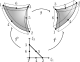
\includegraphics[width=.4\linewidth]{Figuras/Mapeamento.pdf}
    \\Fonte: Autoria Própria (\the\year).
    \label{fig:Mapeamento}
\end{figure}

Para isso, realiza-se primeiramente o mapeamento dos pontos da superfície média do elemento para a configuração inicial de coordenadas $\BB{x}^m$ e para a configuração atual, de coordenadas $\BB{y}^m$:

\begin{subequations}
    \begin{align}
         & \BB{f}^{m0}=\BB{x}^m=\BB{X}_aN_a(\xi_1,\xi_2)\text{,} \\
         & \BB{f}^{m1}=\BB{y}^m=\BB{Y}_aN_a(\xi_1,\xi_2)\text{,}
    \end{align}
\end{subequations}

\noindent onde $\BB{f}^{m0}$ e $\BB{f}^{m1}$ são as funções de mapeamento da superfície média para as configurações inicial a atual, respectivamente, $\BB{X}_a$ e $\BB{Y}_a$ são as coordenadas dos nós $a$, pertencentes à superfície média nas configurações inicial e atual, respectivamente, e $N_a(\xi_1,\xi_2)$ é a função de forma associada ao nó $a$.

Já os pontos fora da superfície média, são mapeados com auxílio de vetores generalizados $\BB{v}^0$ e $\BB{v}^1$, sendo as funções de mapeamento para qualquer ponto, para as configurações inicial e atual, dadas por:

\begin{subequations}
    \begin{align}
         & \BB{f}^0=\BB{x}^m(\xi_1,\xi_2)+\BB{v}^0(\xi_1,\xi_2,\xi_3)\text{ e} \\
         & \BB{f}^1=\BB{y}^m(\xi_1,\xi_2)+\BB{v}^1(\xi_1,\xi_2,\xi_3)\text{,}
    \end{align}
\end{subequations}

\noindent onde $\BB{v}^0$ é normal à superfície média inicial ao ponto mapeado, e enquanto $\BB{v}^1$ é o vetor, não necessariamente normal à superfície média, que liga o ponto da superfície média de coordenadas $(\xi_1,\xi_2)$ ao ponto mapeado na configuração atual. Empregando-se as mesmas funções de forma do elemento plano para representar esses vetores, escrevem-se as aproximações:

\begin{subequations}
    \begin{align}
         & \BB{v}^0=\frac{h_0}{2}\BB{w}^0\xi_3\text{ e}                \\
         & \BB{v}^1=\frac{h_0}{2}\BB{w}^1[\xi_3+\alpha\xi_3^2]\text{,}
    \end{align}
\end{subequations}

\noindent sendo $h_0$ a espessura inicial da casca, $\BB{w}^0$ e $\BB{w}^1$ os vetores generalizados adimensionais na configuração inicial e atual, respectivamente, e $\alpha$ é um enriquecimento nodal inserido ao problema com a finalidade de evitar travamento volumétrico, o qual representa a taxa de variação linear da deformação na direção da espessura. Essas variáveis podem ser aproximadas via funções de forma como:

\begin{subequations}
    \begin{align}
         & \BB{w}^0(\xi_1,\xi_2)=\BB{V}^0_aN_a(\xi_1,\xi_2)\text{,}  \\
         & \BB{w}^1(\xi_1,\xi_2)=\BB{V}^1_aN_a(\xi_1,\xi_2)\text{ e} \\
         & \alpha(\xi_1,\xi_2)=\Alpha_aN_a(\xi_1,\xi_2)\text{,}
    \end{align}
\end{subequations}

\noindent em que $\BB{V}^0_a$, $\BB{V}^1_a$ e $\Alpha_a$ são os valores nodais das variáveis associados ao nó $a$ \cite{sanches2013unconstrained,sanches2014fluid}. É importante notar que $\BB{w}^0$ é unitário e normal à superfície média, enquanto $\BB{w}^1$ não é mais necessariamente normal à superfície média nem unitário.

Sendo assim, o problema possui como graus de liberdade as posições nodais atuais da superfície média ($\BB{Y}_a$), os valores nodais do vetor generalizado adimensional na configuração atual ($\BB{V}^1_a$) e o valor nodal da taxa de variação linear de deformação na direção da espessura ($\Alpha_a$).

Além disso, torna-se necessário determinar o gradiente da função de mudança de configuração. Para isso note que $\BB{f}(\BB{x},t)=\BB{f}^1((\BB{f}^0)^{-1},t)$, portanto é possível se obter o gradiente da função de mudança de configuração ($\BB{A}=\Nx\BB{f}$) como $\BB{A}=\BB{A}^1\cdot(\BB{A}^0)^{-1}$, em que $\BB{A}^0=\Nxi\BB{f}^0$ e $\BB{A}^1=\Nxi\BB{f}^1$.

Considerando-se o princípio da conservação da energia, tem-se:

\begin{equation}
    \delta\Pi=\der{\Pi_0}{\BB{g}}\cdot\delta\BB{g}=0\text{,}
\end{equation}

\noindent em que $\BB{g}$ representa o vetor que contém todos os graus de liberdade do problema. Dada a arbitrarieade de $\delta\BB{g}$, o princípio da estacionariedade da energia escrito em função das posições nodais e vetores generalizados fica:

\begin{subequations}
    \begin{equation}
        \der{\Pi_0}{\BB{Y}_a}=\der{\mathbb{U}}{\BB{Y}_a}+\intDomi{\rho_0\ddBB{y}N_a}-\BB{F}_a-\intFronti{\BB{t}N_a}=\BB{0}\text{,}
    \end{equation}
    \begin{equation}
        \der{\Pi_0}{\BB{V}^1_a}=\der{\mathbb{U}}{\BB{V}^1_a}+\intDomi{\rho_0\frac{h_0}{2}(\xi_3+\alpha\xi_3^2)\ddBB{y}N_a}=\BB{0}\text{,}
    \end{equation}
    \begin{equation}
        \der{\Pi_0}{\Alpha^a}=\der{\mathbb{U}}{\Alpha^a}+\intDomi{\rho_0\frac{h_0}{2}N_a\xi_3^2(\BB{w}^1\cdot\ddBB{y})}=0\text{,}
    \end{equation}
\end{subequations}

\noindent sendo possível definir um vetor resíduo $\BB{r}$ como:

\begin{equation}
    \BB{r}_a(\BB{Y},\BB{V}^1,\BB{\Alpha})=\BB{F}_a^\mathrm{int}+\BB{F}_a^\mathrm{inerc}-\BB{F}_a^\mathrm{ext}=\BB{0}\text{,}
    \label{eq:CSD-g}
\end{equation}

\noindent sendo $\BB{F}_a^\mathrm{int}$ o vetor nodal equivalente de forças internas, $\BB{F}_a^\mathrm{inerc}$ o vetor nodal equivalente de forças inerciais e $\BB{F}_a^\mathrm{ext}$ o vetor nodal equivalente de forças externas, assumidas conservativas, tal que:

\begin{subequations}
    \begin{align}
         & \BB{F}_a^\mathrm{int}=\intDomi{\der{u_e}{\BB{g}_a}}=\intDomi{\BB{S}:\der{\mathbb{E}}{\BB{g}_a}}\text{,}\label{eq:CSD-Fint}           \\
         & \BB{F}_a^\mathrm{inerc}=\intDomi{\rho_0\der{\BB{y}}{\BB{g}_a}\cdot\ddBB{y}}\text{ e}\label{eq:CSD-Finerc}                            \\
         & \BB{F}_a^\mathrm{ext}=\BB{F}_b\cdot\der{\BB{Y}_b}{\BB{g}_a}+\intFronti{\BB{t}\cdot\der{\BB{y}^m}{\BB{g}^a}}\text{.}\label{eq:CSD-Fc}
    \end{align}
    \label{eq:CSD-F}
\end{subequations}

Portanto o problema a ser resolvido é descrito como: determinar $\BB{Y}$, $\BB{V}^1$ e $\BB{\Alpha}$ tais que $\BB{r}(\BB{Y},\BB{V}^1,\BB{\Alpha})=\BB{0}$.

Como é possível perceber, o cálculo de $\BB{r}$ é dependente não somente dos graus de liberdade, mas também das derivadas temporais de $\BB{y}$. Sendo assim, se faz necessária a consideração de um integrador temporal, o qual será utilizado o integrador temporal de Newmark, devido à capacidade de respeitar a conservação de momento linear para $\gamma=1/2$ e apresentando bons resultados para modelagem de elementos de casca, conforme apresentado por \citeonline{sanches2013unconstrained}.
%\textcolor{red}{ Pode deixar o Newmark mesmo para a qualificação, mas vamos mudar isso para o alfa generalizado. Não faz mais sentido usar Newmark.}

A aproximação realizada pelo integrador de Newmark é dada por:

\begin{subequations}
    \begin{equation}
        g_i^{n+1}=g_i^n+\dot{g}_i^n\Delta t+\Delta t^2\bigpar{\bigpar{\frac{1}{2}-\beta}\ddot{g}_i^n+\beta\ddot{g}_i^{n+1}}\text{ e}
    \end{equation}
    \begin{equation}
        \dot{g}_i^{n+1}=\dot{g}_i^n+\Delta t(1-\gamma)\ddot{g}_i^n+\gamma\ddot{g}_i^{n+1}\Delta t\text{,}
    \end{equation}
\end{subequations}

\noindent sendo o superíndice $n$ e $n+1$ a indicação do passo de tempo analisado ($t_n$ e $t_{n+1}$), $\Delta t$ o intervalo de tempo discretizado e $\beta$ e $\gamma$ parâmetros livres, que devem ser escolhidos de forma a garantir a convergência do método, sendo arbitrados valores de $\beta=1/4$ e $\gamma=1/2$, garantindo a estabilidade incondicional do método \cite{LINDFIELD2019239}.

Isolando-se os termos incógnitos em função de variáveis não derivadas no tempo em $n+1$ e daquelas já conhecidas tem-se:

\begin{subequations}
    \begin{equation}
        \ddot{g}_i^{n+1}=\frac{g_i^{n+1}-g_i^n}{\beta\Delta t^2}-\frac{\dot{g}_i^n}{\beta\Delta t}+\bigpar{1-\frac{1}{2\beta}}\ddot{g}_i^n
    \end{equation}
    \begin{equation}
        \dot{g}_i^{n+1}=\frac{\gamma}{\beta\Delta t}(g_i^{n+1}-g_i^n)+\bigpar{1-\frac{\gamma}{\beta}}\dot{g}_i^n+\Delta t\bigpar{1-\frac{\gamma}{2\beta}}\ddot{g}_i^n\text{.}
    \end{equation}
    \label{eq:CSD-Newmark2}
\end{subequations}

Já para procurar valores de $\BB{g}$ que anulem $\BB{r}$, utiliza-se o Método de Newton-Raphson, o qual parte da aproximação por série de Taylor truncada no termo de primeira ordem:

\begin{equation}
    \begin{split}
        &\BB{r}(\BB{g}+\Delta\BB{g})=\BB{r}(\BB{g})+\apderp{\BB{r}}{\BB{g}}{\BB{g}}\Delta\BB{g}=\\
        &\BB{r}(\BB{Y},\BB{V}^1,\BB{\Alpha})+\apderp{\BB{r}}{\BB{Y}}{\BB{Y}}\Delta\BB{Y}+\apderp{\BB{r}}{\BB{V}^1}{\BB{V}^1}\Delta\BB{V}^1+\apderp{\BB{r}}{\BB{\Alpha}}{\BB{\Alpha}}\Delta\BB{\Alpha}=\BB{0}\text{.}
    \end{split}
\end{equation}

\noindent Dessa forma, necessita-se do cálculo de uma matriz Hessiana ($H_{ij}^{ab}$):

\begin{equation}
    H_{ij}^{ab}=\frac{\partial^2\Pi_0}{\partial g_j^b\partial g_i^a}=\der{r_i^a}{g_j^b}\text{.}
\end{equation}

Substituindo-se as derivadas temporais da aproximação de Newmark em $\BB{r}$ e realizando as devidas simplificações, obtém-se:

\begin{equation}
    H_{ij}^{ab}=(H^\text{est})_{ij}^{ab}+\frac{M_{ij}^{ab}}{\beta\Delta t^2}+\intDom{\rho_0\ddot{y}_k\Dder{y_k}{g_j^b}{g_i^a}}\text{,}
    \label{eq:CSD-Hijab}
\end{equation}

\noindent sendo $(H^\text{est})_{ij}^{ab}$ a matriz hessiana estática elementar, $M_{ij}^{ab}$ a matriz de massa e $C_{ij}^{ab}$ a matriz de amortecimento, dadas por:

\begin{subequations}
    \begin{align}
         & (H^\text{est})_{ij}^{ab}=\Dder{\mathbb{U}}{g_j^b}{g_i^a}=\intDomi{\bigpar{\der{S_{kl}}{g_j^b}\der{\mathbb{E}_{kl}}{g_i^a}+S_{kl}\Dder{\mathbb{E}_{kl}}{g_i^a}{g_j^b}}}\text{ e} \\
         & M_{ij}^{ab}=\intDomi{\rho_0\der{y_k}{g_i^a}\der{y_k}{g_j^b}}\text{.}
    \end{align}
    \label{eq:CSD-HMC}
\end{subequations}

\noindent também observa-se que a derivada mista de $y_k$ em relação a $g_i^a$ e $g_j^b$ possuirá valores não-nulos apenas quando for derivada de forma cruzada em relação a $V^1$ e $\Alpha$.

Com isso, encontra-se um vetor de correções dos graus de liberdade ($\Delta\BB{g}$) como a solução do sistema:

\begin{equation}
    H_{ij}\Delta g_j=-r_i\text{,}
\end{equation}

\noindent tendo como critério de parada a medida do erro:

\begin{equation}
    \frac{\norm{\Delta\BB{Y}}}{\norm{\BB{X}}}\leq\text{tol,}
    \label{eq:CSD-erro}
\end{equation}

\noindent em que $\BB{X}$ o vetor de posições nodais iniciais e tol uma tolerância admitida.

%%==================================================================================================
%\subsection{Procedimento Computacional} \label{MEFP-Comp}
%%==================================================================================================
%
%Para a implementação computacional realizou-se uma integração em $\Omega_0$ e $\Gamma_0$ segundo a quadratura de hammer \cite{hammer1956numerical}, sendo a malha gerada %automaticamente via comunicação direta do algoritmo com o \textit{Gmsh} e o procedimento paralelizado utilizando o protocolo MPI presente na biblioteca PETSc. Demais informações %relevantes à implementação computacional são descritas detalhadamente no capítulo \ref{MetodologiaCronograma}.
%
%O algoritmo visto no Apêndice \ref{Ap:Shell-alg} apresentado na forma de pseudocódigo exemplifica o código implementado.

%==================================================================================================
\subsection{Exemplos de Verificação} \label{MEFP-Ex}
%==================================================================================================

Para o melhor conhecimento e para verificação do código a ser utilizado para a dinâmica das estruturas, foram selecionados e simulados os problemas estáticos de \textit{Scordelis-Lo roof} e de um cilindro elástico biengastado, e os problemas dinâmicos de uma viga em balanço e de uma viga bi-engastada submetidas a carregamento de impacto. Tais simulações executadas, contendo os parâmetros de entrada, assim como a discretização de cada problema e os resultados obtidos, são apresentados no Apêndice \ref{Ap:CSD-Exemplos}. %\ref{Ap:SLR}, \ref{Ap:Shell-cyl} e \ref{Ap:DinBeam}, para os respectivos problemas.